% !TEX program = xelatex
% !TEX encoding = UTF-8 Unicode
% =====================================================================
%  Homework 4.1 — Data Warehouse Design: DAKDL Airways
%  Minimal version — covers only what the brief requires. All pages portrait.
%  MUST compile with XeLaTeX (Thai fonts).
% =====================================================================
\documentclass[11pt]{article}

\usepackage{fontspec}
\usepackage[a4paper,margin=1.8cm]{geometry}
\usepackage{underscore}                 % lets snake_case print literally
\usepackage{tikz}
\usetikzlibrary{positioning,shapes.multipart,arrows.meta}
\usepackage{xcolor}
\usepackage{booktabs}
\usepackage{tabularx}
\usepackage{array}
\usepackage{colortbl}
\usepackage{enumitem}
\usepackage{fancyvrb}
\usepackage{graphicx}
\usepackage{adjustbox}
\usepackage[hidelinks]{hyperref}

% ---- Fonts (ONE font for everything: Thai + Latin + code + SQL) ------
\setmainfont{Waree}
\setmonofont{Waree}

% Thai has no spaces between words -> enable ICU dictionary line breaking
\XeTeXlinebreaklocale "th"
\XeTeXlinebreakskip = 0pt plus 0.1em minus 0.05em

% ---- Colours (monochrome) --------------------------------------------
\definecolor{factHead}{gray}{0.18}
\definecolor{factBody}{gray}{0.90}
\definecolor{dimHead}{gray}{0.40}
\definecolor{dimBody}{gray}{0.95}
\definecolor{tblHead}{gray}{0.28}
\definecolor{tblAlt}{gray}{0.93}
\definecolor{accent}{gray}{0.00}
\definecolor{codeframe}{gray}{0.55}

% ---- Helpers ---------------------------------------------------------
\newcommand{\code}[1]{\texttt{#1}}
\newcommand{\PK}{\textbf{\textcolor{accent}{PK}}}
\newcommand{\FK}{\textbf{\textcolor{factHead}{FK}}}
\newcommand{\secline}{\par\vspace{-2pt}\noindent\textcolor{tblHead}{\rule{\linewidth}{0.8pt}}\par\vspace{3pt}}

\usepackage{titlesec}
\titleformat{\section}{\large\bfseries\color{factHead}}{\thesection.}{0.5em}{}
\titlespacing*{\section}{0pt}{9pt}{4pt}
\titleformat{\subsection}{\normalsize\bfseries\color{tblHead}}{\thesubsection}{0.5em}{}
\titlespacing*{\subsection}{0pt}{6pt}{3pt}

% SQL block style
\DefineVerbatimEnvironment{sql}{Verbatim}%
  {fontsize=\footnotesize,frame=single,framesep=4pt,rulecolor=\color{codeframe},%
   xleftmargin=3pt,xrightmargin=3pt}

\newcolumntype{Y}{>{\raggedright\arraybackslash}X}

% Attribute-table header row (Attribute / Type / Description).
% NOTE: plain `tabular`, not tabularx — tabularx scans the input stream for a
% literal \end{tabularx}, so it cannot be split across a custom environment.
\newcommand{\atthead}{\rowcolor{tblHead}
  \textcolor{white}{\textbf{Attribute}} & \textcolor{white}{\textbf{Data Type}} & \textcolor{white}{\textbf{คำอธิบาย}}\\}
\newenvironment{atttable}[1]%
  {\subsection*{#1}\vspace{-4pt}
   \begin{tabular}{@{}>{\ttfamily\small}p{4.3cm} >{\small}p{2.7cm} >{\small\raggedright\arraybackslash}p{9.4cm}@{}}
   \toprule\atthead \midrule}%
  {\bottomrule\end{tabular}\vspace{3pt}}

\begin{document}

% =====================================================================
\begin{center}
  {\LARGE\bfseries\color{factHead} การออกแบบคลังข้อมูล DAKDL Airways}\\[4pt]
  {\small Homework 4.1 \quad|\quad รหัสนักศึกษา 6710503739}
\end{center}
\secline

% =====================================================================
\section{Business Processes, Granularities, Dimensions, Measures}
% =====================================================================

\subsection*{1.1 Business Processes}
\begin{enumerate}[leftmargin=16pt,itemsep=1pt,topsep=2pt]
  \item \textbf{Flight Operations} — การดำเนินงานเที่ยวบิน (ความตรงต่อเวลา, ความล่าช้า, ความเต็มของเที่ยวบิน)
  \item \textbf{Booking Revenue} — รายได้จากการจอง (รายได้, ราคาตั๋ว, การจองล่วงหน้า, ความภักดีของลูกค้า)
\end{enumerate}

\subsection*{1.2 Granularities}
\begin{tabularx}{\linewidth}{@{}>{\small}p{4.3cm} Y@{}}
\toprule
\rowcolor{tblHead}
\textcolor{white}{\textbf{Fact Table}} & \textcolor{white}{\textbf{1 แถว แทนอะไร?}}\\
\midrule
\code{Fact_Flight_Operations} & 1 เที่ยวบิน (flight leg) ที่ทำการบินจริง 1 ครั้ง ในวันที่ระบุ\\

\code{Fact_Booking_Revenue} & การจอง 1 รายการ ของผู้โดยสาร 1 คน บนเที่ยวบิน 1 เที่ยว ในชั้นที่นั่ง 1 ชั้น\\
\bottomrule
\end{tabularx}

\clearpage
% =====================================================================
\section{ผัง Star Schema}
% =====================================================================
\vspace{-2pt}
\begin{center}
% Portrait layout: conformed dimensions sit in a middle row between the two
% stacked fact tables, so the diagram is taller than it is wide.
\resizebox{\linewidth}{!}{%
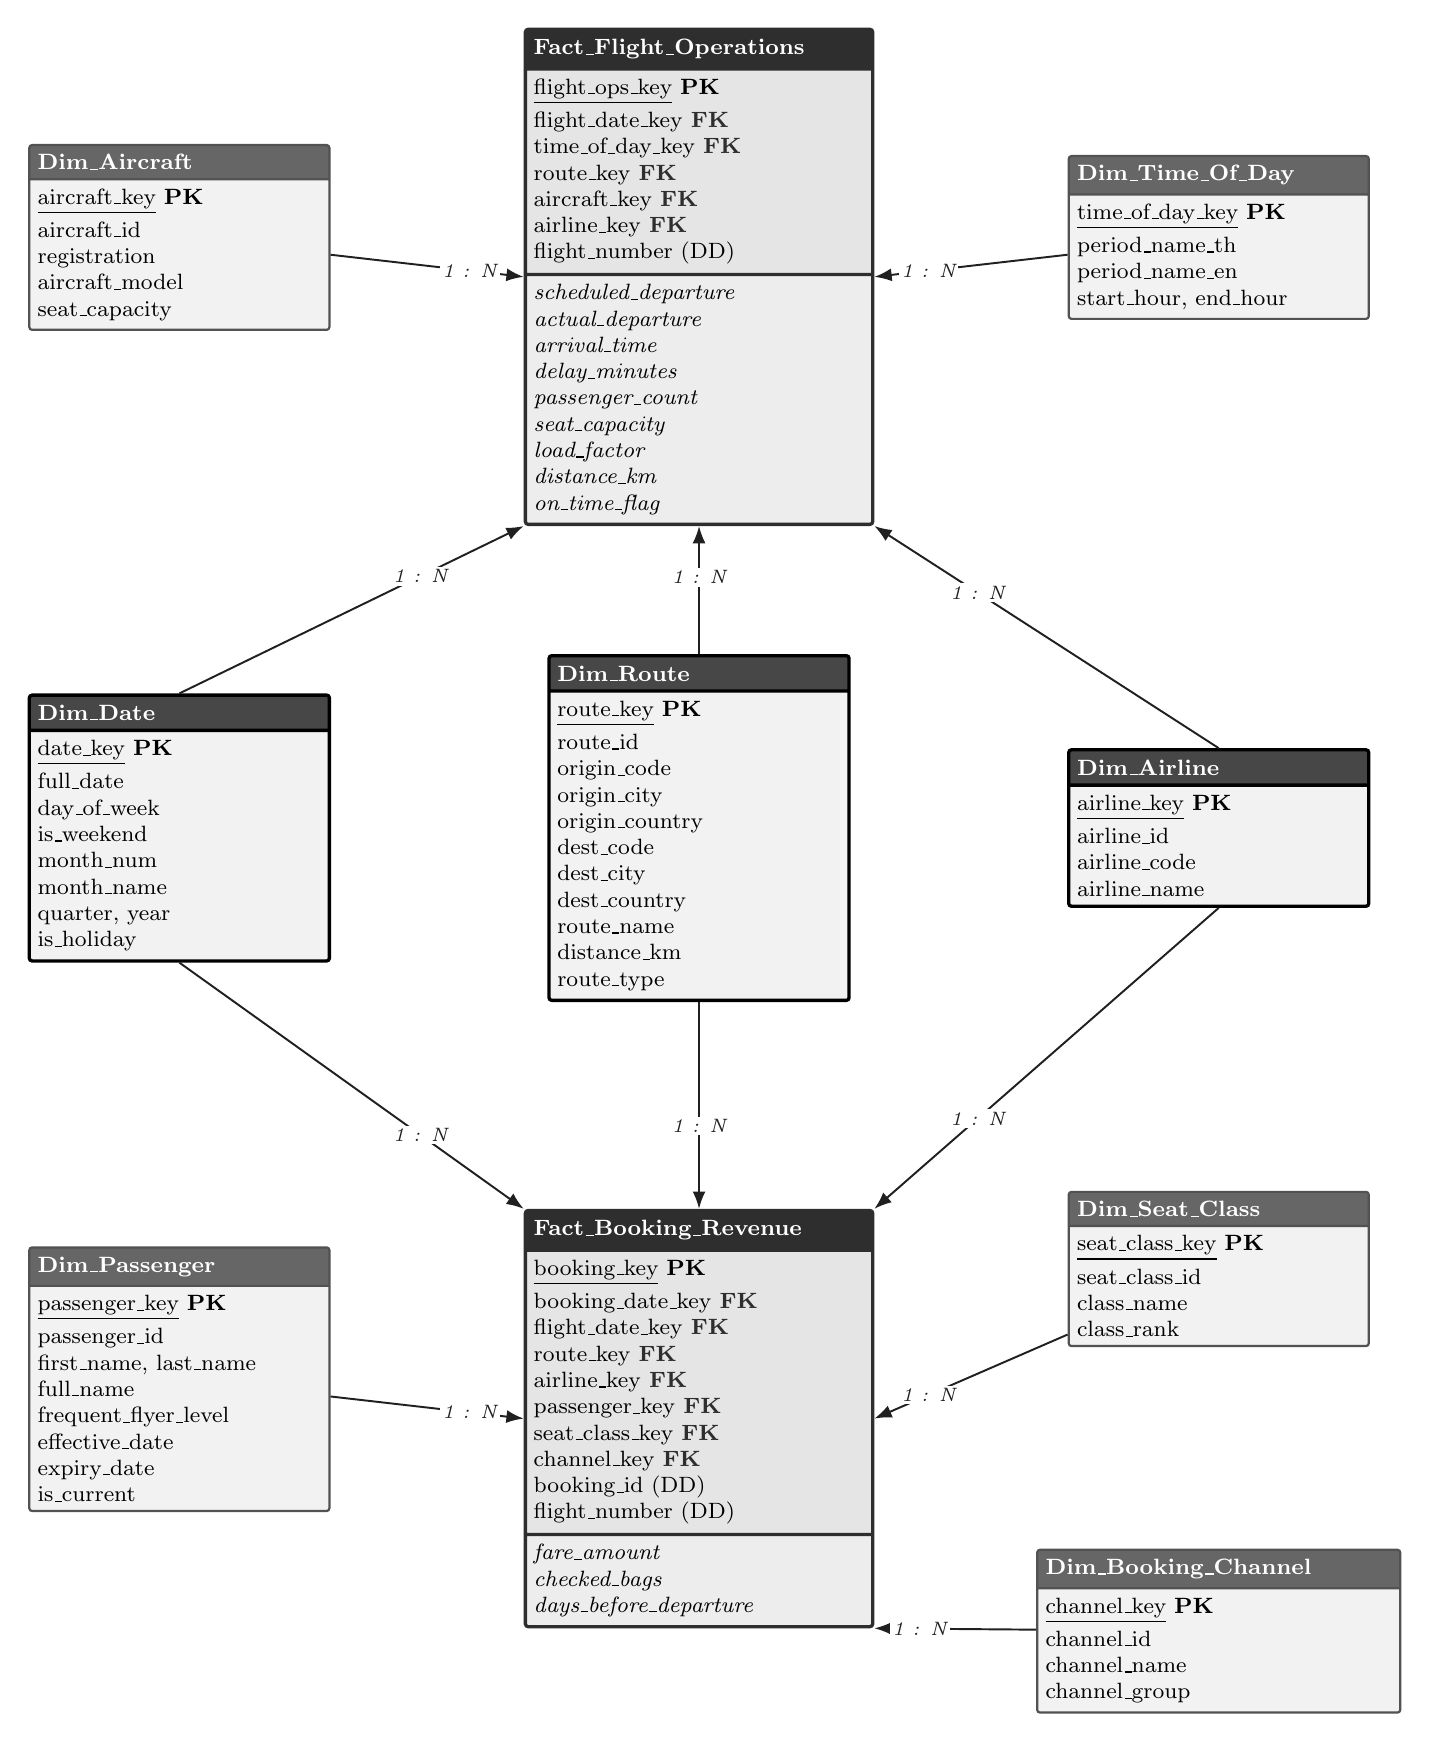
\begin{tikzpicture}[
  every node/.style={font=\footnotesize},
  tbl/.style={draw=dimHead!80!black, line width=0.8pt, rounded corners=1pt,
      rectangle split, rectangle split parts=2,
      rectangle split part fill={dimHead, dimBody},
      text width=3.6cm, align=left, inner sep=3pt},
  shared/.style={tbl, draw=accent, line width=1.2pt,
      rectangle split part fill={tblHead, dimBody}},
  facttbl/.style={draw=factHead, line width=1.2pt, rounded corners=1pt,
      rectangle split, rectangle split parts=3,
      rectangle split part fill={factHead, factBody, factBody!70!white},
      text width=4.2cm, align=left, inner sep=3pt},
  rel/.style={-{Latex[length=2.2mm]}, line width=0.7pt, factHead!70!black},
  hdr/.style={text=white},
  lbl/.style={font=\scriptsize\itshape, fill=white, inner sep=1pt}
]

% ---------- FACT 1 (top) ----------
\node[facttbl] (f1) at (-3,7) {
  \nodepart[hdr]{one}\textbf{Fact_Flight_Operations}
  \nodepart{two}
    \underline{flight_ops_key} \PK\\[2.5pt]
    flight_date_key \FK\\ time_of_day_key \FK\\ route_key \FK\\
    aircraft_key \FK\\ airline_key \FK\\ flight_number (DD)
  \nodepart{three}
    \textit{scheduled_departure}\\ \textit{actual_departure}\\ \textit{arrival_time}\\
    \textit{delay_minutes}\\ \textit{passenger_count}\\ \textit{seat_capacity}\\
    \textit{load_factor}\\ \textit{distance_km}\\ \textit{on_time_flag}
};

% ---------- FACT 2 (bottom) ----------
\node[facttbl] (f2) at (-3,-7.5) {
  \nodepart[hdr]{one}\textbf{Fact_Booking_Revenue}
  \nodepart{two}
    \underline{booking_key} \PK\\[2.5pt]
    booking_date_key \FK\\ flight_date_key \FK\\ route_key \FK\\
    airline_key \FK\\ passenger_key \FK\\ seat_class_key \FK\\
    channel_key \FK\\ booking_id (DD)\\ flight_number (DD)
  \nodepart{three}
    \textit{fare_amount}\\ \textit{checked_bags}\\
    \textit{days_before_departure}
};

% ---------- CONFORMED DIMENSIONS (middle row, shared by both facts) ----------
\node[shared] (date) at (-9.6,0) {
  \nodepart[hdr]{one}\textbf{Dim_Date}\\ 
  \nodepart{two}\underline{date_key} \PK\\[2.5pt] full_date\\ day_of_week\\ is_weekend\\ month_num\\ month_name\\ quarter, year\\ is_holiday};
\node[shared] (route) at (-3,0) {
  \nodepart[hdr]{one}\textbf{Dim_Route}\\ 
  \nodepart{two}\underline{route_key} \PK\\[2.5pt] route_id\\ origin_code\\ origin_city\\ origin_country\\ dest_code\\ dest_city\\ dest_country\\ route_name\\ distance_km\\ route_type};
\node[shared] (airline) at (3.6,0) {
  \nodepart[hdr]{one}\textbf{Dim_Airline}\\
  \nodepart{two}\underline{airline_key} \PK\\[2.5pt] airline_id\\ airline_code\\ airline_name};

% ---------- FACT 1 ONLY ----------
\node[tbl] (aircraft) at (-9.6,7.5) {
  \nodepart[hdr]{one}\textbf{Dim_Aircraft}
  \nodepart{two}\underline{aircraft_key} \PK\\[2.5pt] aircraft_id\\ registration\\ aircraft_model\\ seat_capacity};
\node[tbl] (tod) at (3.6,7.5) {
  \nodepart[hdr]{one}\textbf{Dim_Time_Of_Day}
  \nodepart{two}\underline{time_of_day_key} \PK\\[2.5pt] period_name_th\\ period_name_en\\ start_hour, end_hour};

% ---------- FACT 2 ONLY ----------
\node[tbl] (pax) at (-9.6,-7.0) {
  \nodepart[hdr]{one}\textbf{Dim_Passenger} 
  \nodepart{two}\underline{passenger_key} \PK\\[2.5pt] passenger_id\\ first_name, last_name\\ full_name\\ frequent_flyer_level\\ effective_date\\ expiry_date\\ is_current};
\node[tbl] (seat) at (3.6,-5.6) {
  \nodepart[hdr]{one}\textbf{Dim_Seat_Class}
  \nodepart{two}\underline{seat_class_key} \PK\\[2.5pt] seat_class_id\\ class_name\\ class_rank};
\node[tbl, text width=4.4cm] (chan) at (3.6,-10.2) {
  \nodepart[hdr]{one}\textbf{Dim_Booking_Channel}
  \nodepart{two}\underline{channel_key} \PK\\[2.5pt] channel_id\\ channel_name\\ channel_group};

% ---------- RELATIONSHIPS ----------
\draw[rel] (date.north)    -- node[lbl,pos=0.7]{1 : N} (f1.south west);
\draw[rel] (date.south)    -- node[lbl,pos=0.7]{1 : N} (f2.north west);
\draw[rel] (route.north)   -- node[lbl,pos=0.6]{1 : N} (f1.south);
\draw[rel] (route.south)   -- node[lbl,pos=0.6]{1 : N} (f2.north);
\draw[rel] (airline.north) -- node[lbl,pos=0.7]{1 : N} (f1.south east);
\draw[rel] (airline.south) -- node[lbl,pos=0.7]{1 : N} (f2.north east);
\draw[rel] (aircraft)      -- node[lbl,pos=0.72]{1 : N} (f1.west);
\draw[rel] (tod)           -- node[lbl,pos=0.72]{1 : N} (f1.east);
\draw[rel] (pax)           -- node[lbl,pos=0.72]{1 : N} (f2.west);
\draw[rel] (seat)          -- node[lbl,pos=0.72]{1 : N} (f2.east);
\draw[rel] (chan)          -- node[lbl,pos=0.72]{1 : N} (f2.south east);
\end{tikzpicture}}
\end{center}

\vspace{2pt}
\noindent\small
\textbf{คำอธิบาย:} ใช้ 2 Fact Tables เพราะทั้งสองกระบวนการมี grain ต่างกัน
กล่องสีเข้มตรงกลาง (\mbox{\code{Dim_Date}}, \mbox{\code{Dim_Route}}, \mbox{\code{Dim_Airline}}) เป็น Conformed Dimensions
ที่ใช้ร่วมกันทั้ง 2 Fact โดย \code{Dim_Date} ใช้ 2 บทบาทใน Fact 2 (วันที่จอง / วันที่บิน)
ส่วน \code{flight_number} และ \code{booking_id} เป็น Degenerate Dimension เก็บไว้ใน Fact โดยตรง
\normalsize

\clearpage
% =====================================================================
\section{คำอธิบาย Attribute (Data Type + Description)}
% =====================================================================

\begin{atttable}{3.1 \ Fact_Flight_Operations}
flight_ops_key      & INT (PK)      & คีย์ของแถว\\
flight_date_key     & INT (FK)      & เชื่อมไป \code{Dim_Date} \\
time_of_day_key     & INT (FK)      & เชื่อมไป \code{Dim_Time_Of_Day} \\
route_key           & INT (FK)      & เชื่อมไป \code{Dim_Route}\\
aircraft_key        & INT (FK)      & เชื่อมไป \code{Dim_Aircraft}\\
airline_key         & INT (FK)      & เชื่อมไป \code{Dim_Airline}\\
flight_number       & VARCHAR(10)   & หมายเลขเที่ยวบิน\\
scheduled_departure & TIME          & เวลาออกเดินทางตามตาราง\\
actual_departure    & TIME          & เวลาออกเดินทางจริง\\
arrival_time        & TIME          & เวลาถึงปลายทาง\\
delay_minutes       & INT           & นาทีที่ล่าช้า\\
passenger_count     & INT           & จำนวนผู้โดยสารจริง\\
seat_capacity       & INT           & ความจุที่นั่งของอากาศยาน\\
load_factor         & DECIMAL(5,4)  & ความเต็มของเที่ยวบิน\\
distance_km         & DECIMAL(8,2)  & ระยะทางบิน \\
on_time_flag        & TINYINT(1)    & 1 = ตรงเวลา, 0 = ล่าช้า\\
\end{atttable}

\begin{atttable}{3.2 \ Fact_Booking_Revenue}
booking_key         & INT (PK)      & คีย์ของแถว\\
booking_date_key    & INT (FK)      & เชื่อมไป \code{Dim_Date} \\
flight_date_key     & INT (FK)      & เชื่อมไป \code{Dim_Date} \\
route_key           & INT (FK)      & เชื่อมไป \code{Dim_Route}\\
airline_key         & INT (FK)      & เชื่อมไป \code{Dim_Airline}\\
passenger_key       & INT (FK)      & เชื่อมไป \code{Dim_Passenger}\\
seat_class_key      & INT (FK)      & เชื่อมไป \code{Dim_Seat_Class}\\
channel_key         & INT (FK)      & เชื่อมไป \code{Dim_Booking_Channel}\\
booking_id          & INT           & รหัสการจอง\\
flight_number       & VARCHAR(10)   & หมายเลขเที่ยวบินที่จอง\\
fare_amount         & DECIMAL(10,2) & ราคาตั๋ว\\
checked_bags        & INT           & จำนวนสัมภาระที่โหลด\\
days_before_departure & INT         & จำนวนวันที่จองล่วงหน้า\\
\end{atttable}

\begin{atttable}{3.3 \ Dim_Date }
date_key    & INT (PK)    & คีย์รูปแบบ YYYYMMDD\\
full_date   & DATE        & วันที่จริง\\
day_of_week & VARCHAR(10) & ชื่อวันในสัปดาห์\\
is_weekend  & TINYINT(1)  & 1 = เสาร์/อาทิตย์\\
month_num   & TINYINT     & เลขเดือน 1–12\\
month_name  & VARCHAR(12) & ชื่อเดือน\\
quarter     & TINYINT     & ไตรมาส 1–4\\
year        & SMALLINT    & ปี ค.ศ.\\
is_holiday  & TINYINT(1)  & 1 = วันหยุด\\
\end{atttable}

\begin{atttable}{3.4 \ Dim_Route }
route_key      & INT (PK)     & คีย์ของเส้นทาง\\
route_id       & INT          & รหัสเส้นทาง\\
origin_code    & CHAR(3)      & รหัสสนามบินต้นทาง\\
origin_city    & VARCHAR(50)  & เมืองต้นทาง\\
origin_country & VARCHAR(50)  & ประเทศต้นทาง\\
dest_code      & CHAR(3)      & รหัสสนามบินปลายทาง\\
dest_city      & VARCHAR(50)  & เมืองปลายทาง\\
dest_country   & VARCHAR(50)  & ประเทศปลายทาง\\
route_name     & VARCHAR(20)  & ชื่อย่อเส้นทาง\\
distance_km    & DECIMAL(8,2) & ระยะทางบิน \\
route_type     & VARCHAR(15)  & Domestic / International\\
\end{atttable}

\clearpage
\begin{atttable}{3.5 \ Dim_Passenger }
passenger_key        & INT (PK)     & คีย์ของผู้โดยสาร 1 คนมีได้หลายแถวตามประวัติระดับสมาชิก\\
passenger_id         & INT          & รหัสผู้โดยสาร\\
first_name           & VARCHAR(50)  & ชื่อ\\
last_name            & VARCHAR(50)  & นามสกุล\\
full_name            & VARCHAR(101) & ชื่อเต็ม\\
frequent_flyer_level & VARCHAR(20)  & ระดับสมาชิก\\
effective_date       & DATE         & วันที่เริ่มมีผลของแถวนี้ (SCD2)\\
expiry_date          & DATE         & วันที่สิ้นสุด ถ้ายังใช้อยู่ = 9999-12-31 (SCD2)\\
is_current           & TINYINT(1)   & 1 = แถวปัจจุบัน, 0 = แถวประวัติ (SCD2)\\
\end{atttable}

\begin{atttable}{3.6 \ Dim_Aircraft \ / \ Dim_Airline \ / \ Dim_Seat_Class \ / \ Dim_Booking_Channel \ / \ Dim_Time_Of_Day}
aircraft_key    & INT (PK)     & คีย์ของเครื่องบิน\\
aircraft_id     & INT          & รหัสเครื่องบิน\\
registration    & VARCHAR(20)  & ทะเบียนเครื่องบิน\\
aircraft_model  & VARCHAR(50)  & รุ่นเครื่องบิน\\
seat_capacity   & INT          & จำนวนที่นั่งทั้งหมด\\
\midrule
airline_key     & INT (PK)     & คีย์ของสายการบิน\\
airline_id      & INT          & รหัสสายการบิน\\
airline_code    & CHAR(2)      & รหัสสายการบิน\\
airline_name    & VARCHAR(100) & ชื่อสายการบิน\\
\midrule
seat_class_key  & INT (PK)     & คีย์ของชั้นที่นั่ง\\
seat_class_id   & INT          & รหัสชั้นที่นั่ง\\
class_name      & VARCHAR(30)  & Economy / Business / First\\
class_rank      & TINYINT      & ลำดับชั้น 1=Economy, 2=Business, 3=First\\
\midrule
channel_key     & INT (PK)     & คีย์ของช่องทางการจอง\\
channel_id      & INT          & รหัสช่องทาง\\
channel_name    & VARCHAR(30)  & Online / Phone / Agent\\
channel_group   & VARCHAR(20)  & Direct / Indirect\\
\midrule
time_of_day_key & INT (PK)     & คีย์ของช่วงเวลา\\
period_name_th  & VARCHAR(20)  & เช้า / บ่าย / เย็น / กลางคืน\\
period_name_en  & VARCHAR(20)  & Morning / Afternoon / Evening / Night\\
start_hour      & TINYINT      & ชั่วโมงเริ่มต้นของช่วง\\
end_hour        & TINYINT      & ชั่วโมงสิ้นสุดของช่วง\\
\end{atttable}

\clearpage
% =====================================================================
\section{ตัวอย่างข้อมูลสมมุติ (Sample Data)}
% =====================================================================
\noindent\small ไฟล์ CSV แนบในโฟลเดอร์ \code{sample_data/}\normalsize
\vspace{4pt}

\subsection*{4.1 \ Dim_Date}
{\footnotesize
\begin{adjustbox}{max width=\linewidth}
\begin{tabular}{@{}l l l c c l c c c@{}}
\toprule
\rowcolor{tblHead}
\textcolor{white}{date_key} & \textcolor{white}{full_date} & \textcolor{white}{day_of_week} &
\textcolor{white}{is_weekend} & \textcolor{white}{month_num} & \textcolor{white}{month_name} &
\textcolor{white}{quarter} & \textcolor{white}{year} & \textcolor{white}{is_holiday}\\
\midrule
20240301 & 2024-03-01 & Friday   & 0 & 3 & March & 1 & 2024 & 0\\
20240302 & 2024-03-02 & Saturday & 1 & 3 & March & 1 & 2024 & 0\\
20240305 & 2024-03-05 & Tuesday  & 0 & 3 & March & 1 & 2024 & 0\\
20240308 & 2024-03-08 & Friday   & 0 & 3 & March & 1 & 2024 & 0\\
20240309 & 2024-03-09 & Saturday & 1 & 3 & March & 1 & 2024 & 0\\
20240310 & 2024-03-10 & Sunday   & 1 & 3 & March & 1 & 2024 & 0\\
20240312 & 2024-03-12 & Tuesday  & 0 & 3 & March & 1 & 2024 & 0\\
20240314 & 2024-03-14 & Thursday & 0 & 3 & March & 1 & 2024 & 0\\
20240315 & 2024-03-15 & Friday   & 0 & 3 & March & 1 & 2024 & 0\\
\bottomrule
\end{tabular}
\end{adjustbox}}

\subsection*{4.2 \ Dim_Route}
{\footnotesize
\begin{adjustbox}{max width=\linewidth}
\begin{tabular}{@{}c c l l l c l l l r l@{}}
\toprule
\rowcolor{tblHead}
\textcolor{white}{route_key} & \textcolor{white}{route_id} & \textcolor{white}{origin_code} &
\textcolor{white}{origin_city} & \textcolor{white}{origin_country} & \textcolor{white}{dest_code} &
\textcolor{white}{dest_city} & \textcolor{white}{dest_country} &
\textcolor{white}{route_name} & \textcolor{white}{distance_km} & \textcolor{white}{route_type}\\
\midrule
1 & 101 & BKK & Bangkok & Thailand & CNX & Chiang Mai & Thailand  & BKK-CNX & 588.00 & Domestic\\
2 & 102 & BKK & Bangkok & Thailand & HKT & Phuket     & Thailand  & BKK-HKT & 689.00 & Domestic\\
3 & 103 & BKK & Bangkok & Thailand & NRT & Tokyo      & Japan     & BKK-NRT & 4610.00 & International\\
4 & 104 & BKK & Bangkok & Thailand & SIN & Singapore  & Singapore & BKK-SIN & 1424.00 & International\\
\bottomrule
\end{tabular}
\end{adjustbox}}

\subsection*{4.3 \ Dim_Aircraft \ , \ Dim_Time_Of_Day \ , \ Dim_Seat_Class \ , \ Dim_Booking_Channel \ , \ Dim_Airline}
{\footnotesize
\begin{minipage}[t]{0.49\linewidth}
\begin{adjustbox}{max width=\linewidth}
\begin{tabular}{@{}c c l l c@{}}
\toprule
\rowcolor{tblHead}
\textcolor{white}{aircraft_key} & \textcolor{white}{a_id} & \textcolor{white}{registration} &
\textcolor{white}{aircraft_model} & \textcolor{white}{cap}\\
\midrule
1 & 501 & HS-DAK1 & Airbus A320    & 180\\
2 & 502 & HS-DAK2 & Boeing 737-800 & 189\\
3 & 503 & HS-DAK5 & Boeing 787-9   & 298\\
\bottomrule
\end{tabular}
\end{adjustbox}
\vspace{6pt}

\begin{adjustbox}{max width=\linewidth}
\begin{tabular}{@{}c l l c c@{}}
\toprule
\rowcolor{tblHead}
\textcolor{white}{tod_key} & \textcolor{white}{period_th} & \textcolor{white}{period_en} &
\textcolor{white}{start} & \textcolor{white}{end}\\
\midrule
1 & เช้า     & Morning   & 5  & 11\\
2 & บ่าย     & Afternoon & 12 & 16\\
3 & เย็น     & Evening   & 17 & 20\\
4 & กลางคืน & Night     & 21 & 4\\
\bottomrule
\end{tabular}
\end{adjustbox}
\end{minipage}\hfill
\begin{minipage}[t]{0.49\linewidth}
\begin{adjustbox}{max width=\linewidth}
\begin{tabular}{@{}c c l c@{}}
\toprule
\rowcolor{tblHead}
\textcolor{white}{seat_class_key} & \textcolor{white}{sc_id} & \textcolor{white}{class_name} &
\textcolor{white}{class_rank}\\
\midrule
1 & 11 & Economy  & 1\\
2 & 12 & Business & 2\\
3 & 13 & First    & 3\\
\bottomrule
\end{tabular}
\end{adjustbox}
\vspace{6pt}

\begin{adjustbox}{max width=\linewidth}
\begin{tabular}{@{}c c l l@{}}
\toprule
\rowcolor{tblHead}
\textcolor{white}{channel_key} & \textcolor{white}{ch_id} & \textcolor{white}{channel_name} &
\textcolor{white}{channel_group}\\
\midrule
1 & 21 & Online & Direct\\
2 & 22 & Phone  & Direct\\
3 & 23 & Agent  & Indirect\\
\bottomrule
\end{tabular}
\end{adjustbox}
\vspace{6pt}

\begin{adjustbox}{max width=\linewidth}
\begin{tabular}{@{}c c l l@{}}
\toprule
\rowcolor{tblHead}
\textcolor{white}{airline_key} & \textcolor{white}{al_id} & \textcolor{white}{code} &
\textcolor{white}{airline_name}\\
\midrule
1 & 1 & DA & DAKDL Airways\\
\bottomrule
\end{tabular}
\end{adjustbox}
\end{minipage}}

\subsection*{4.4 \ Dim_Passenger}
{\footnotesize
\begin{adjustbox}{max width=\linewidth}
\begin{tabular}{@{}c c l l l l c@{}}
\toprule
\rowcolor{tblHead}
\textcolor{white}{passenger_key} & \textcolor{white}{passenger_id} & \textcolor{white}{full_name} &
\textcolor{white}{frequent_flyer_level} & \textcolor{white}{effective_date} &
\textcolor{white}{expiry_date} & \textcolor{white}{is_current}\\
\midrule
1 & 1 & Somchai Jaidee & Silver   & 2022-01-01 & 2023-12-31 & 0\\
2 & 1 & Somchai Jaidee & Gold     & 2024-01-01 & 9999-12-31 & 1\\
3 & 2 & Malee Sukjai   & Silver   & 2023-06-01 & 9999-12-31 & 1\\
4 & 3 & Anan Wongchai  & Platinum & 2023-01-01 & 9999-12-31 & 1\\
5 & 4 & Nita Phromma   & Basic    & 2024-02-01 & 9999-12-31 & 1\\
6 & 5 & John Miller    & Gold     & 2023-03-01 & 9999-12-31 & 1\\
\bottomrule
\end{tabular}
\end{adjustbox}}

\subsection*{4.5 \ Fact_Flight_Operations}
{\footnotesize
\begin{adjustbox}{max width=\linewidth}
\begin{tabular}{@{}c c c c c c l c c c r r r c r c@{}}
\toprule
\rowcolor{tblHead}
\textcolor{white}{ops_key} & \textcolor{white}{fdate} & \textcolor{white}{tod} &
\textcolor{white}{route} & \textcolor{white}{acft} & \textcolor{white}{al} &
\textcolor{white}{flight_no} & \textcolor{white}{sched_dep} & \textcolor{white}{act_dep} &
\textcolor{white}{arr_time} & \textcolor{white}{delay} & \textcolor{white}{pax} &
\textcolor{white}{cap} & \textcolor{white}{load_factor} & \textcolor{white}{distance_km} &
\textcolor{white}{on_time}\\
\midrule
1 & 20240315 & 1 & 1 & 1 & 1 & DA101 & 07:00 & 07:05 & 08:20 &  5 & 162 & 180 & 0.9000 &  588.00 & 1\\
2 & 20240315 & 1 & 2 & 2 & 1 & DA205 & 08:30 & 08:30 & 09:55 &  0 & 170 & 189 & 0.8995 &  689.00 & 1\\
3 & 20240315 & 3 & 3 & 3 & 1 & DA310 & 18:15 & 19:00 & 01:00 & 45 & 265 & 298 & 0.8893 & 4610.00 & 0\\
4 & 20240315 & 2 & 4 & 1 & 1 & DA412 & 13:40 & 14:02 & 16:22 & 22 & 149 & 180 & 0.8278 & 1424.00 & 0\\
5 & 20240315 & 3 & 1 & 2 & 1 & DA103 & 19:20 & 19:32 & 20:47 & 12 & 181 & 189 & 0.9577 &  588.00 & 1\\
6 & 20240315 & 1 & 3 & 3 & 1 & DA311 & 09:50 & 10:50 & 16:50 & 60 & 240 & 298 & 0.8054 & 4610.00 & 0\\
\bottomrule
\end{tabular}
\end{adjustbox}}

\subsection*{4.6 \ Fact_Booking_Revenue}
{\footnotesize
\begin{adjustbox}{max width=\linewidth}
\begin{tabular}{@{}c c c c c c c c c l r c r@{}}
\toprule
\rowcolor{tblHead}
\textcolor{white}{bk_key} & \textcolor{white}{bdate} & \textcolor{white}{fdate} &
\textcolor{white}{route} & \textcolor{white}{al} & \textcolor{white}{pax_key} &
\textcolor{white}{class} & \textcolor{white}{chan} & \textcolor{white}{bk_id} &
\textcolor{white}{flight_no} & \textcolor{white}{fare_amount} & \textcolor{white}{bags} &
\textcolor{white}{days_before}\\
\midrule
1 & 20240301 & 20240315 & 1 & 1 & 2 & 1 & 1 & 9001 & DA101 &  2450.00 & 1 & 14\\
2 & 20240310 & 20240315 & 1 & 1 & 3 & 2 & 2 & 9002 & DA101 &  8900.00 & 2 &  5\\
3 & 20240305 & 20240315 & 3 & 1 & 4 & 2 & 3 & 9003 & DA310 & 42500.00 & 2 & 10\\
4 & 20240312 & 20240315 & 3 & 1 & 2 & 1 & 1 & 9004 & DA310 & 18900.00 & 1 &  3\\
5 & 20240302 & 20240315 & 2 & 1 & 5 & 1 & 1 & 9005 & DA205 &  1990.00 & 0 & 20\\
6 & 20240308 & 20240315 & 4 & 1 & 6 & 1 & 3 & 9006 & DA412 &  5600.00 & 1 & 12\\
7 & 20240314 & 20240315 & 1 & 1 & 2 & 1 & 1 & 9007 & DA103 &  2100.00 & 0 &  1\\
8 & 20240309 & 20240315 & 3 & 1 & 4 & 3 & 2 & 9008 & DA311 & 78000.00 & 3 &  8\\
\bottomrule
\end{tabular}
\end{adjustbox}}

\clearpage
% =====================================================================
\section{Business Questions และ SQL Query (6 ข้อ)}
% =====================================================================

\subsection*{BQ1. รายงาน ``ประสิทธิภาพเที่ยวบินรายวัน'' ของวันที่ 15 มีนาคม 2024}
\begin{sql}
SELECT f.flight_number, r.route_name, a.aircraft_model, t.period_name_en AS time_period,
       f.scheduled_departure, f.actual_departure, f.arrival_time,
       f.delay_minutes, f.passenger_count, f.seat_capacity,
       ROUND(100.0 * f.load_factor, 2) AS load_factor_pct
FROM Fact_Flight_Operations f
JOIN Dim_Date d ON f.flight_date_key = d.date_key
JOIN Dim_Route r ON f.route_key = r.route_key
JOIN Dim_Aircraft a ON f.aircraft_key = a.aircraft_key
JOIN Dim_Time_Of_Day t ON f.time_of_day_key = t.time_of_day_key
WHERE d.full_date = '2024-03-15'
ORDER BY r.route_name, f.scheduled_departure;
\end{sql}

\subsection*{BQ2. แต่ละวันมีเที่ยวบินตรงเวลากี่เที่ยว และล่าช้ากี่เที่ยว?}
\begin{sql}
SELECT d.full_date,
       SUM(f.on_time_flag) AS on_time_flights,
       COUNT(*) - SUM(f.on_time_flag) AS delayed_flights,
       ROUND(100.0 * SUM(f.on_time_flag) / COUNT(*), 1) AS on_time_pct
FROM Fact_Flight_Operations f
JOIN Dim_Date d ON f.flight_date_key = d.date_key
GROUP BY d.full_date
ORDER BY d.full_date;
\end{sql}

\subsection*{BQ3. ค่าเฉลี่ยนาทีที่ล่าช้าตามเส้นทางและช่วงเวลาเป็นอย่างไร?}
\begin{sql}
SELECT r.route_name, t.period_name_en AS time_period,
       COUNT(*) AS num_flights,
       ROUND(AVG(f.delay_minutes), 1) AS avg_delay_min
FROM Fact_Flight_Operations f
JOIN Dim_Route r ON f.route_key = r.route_key
JOIN Dim_Time_Of_Day t ON f.time_of_day_key = t.time_of_day_key
GROUP BY r.route_name, t.period_name_en, t.start_hour
ORDER BY avg_delay_min DESC;
\end{sql}

\subsection*{BQ4. อากาศยานและเส้นทางใดมีประสิทธิภาพดี/แย่ที่สุด (ความเต็มของเที่ยวบิน)?}
\begin{sql}
SELECT a.aircraft_model, r.route_name,
       COUNT(*) AS num_flights,
       SUM(f.passenger_count) AS total_passengers,
       SUM(f.seat_capacity) AS total_seats,
       ROUND(100.0 * SUM(f.passenger_count) / SUM(f.seat_capacity), 2) AS load_factor_pct,
       ROUND(AVG(f.delay_minutes), 1) AS avg_delay_min
FROM Fact_Flight_Operations f
JOIN Dim_Aircraft a ON f.aircraft_key = a.aircraft_key
JOIN Dim_Route r ON f.route_key = r.route_key
GROUP BY a.aircraft_model, r.route_name
ORDER BY load_factor_pct DESC;
\end{sql}
\clearpage
\subsection*{BQ5. รายงาน ``วิเคราะห์รายได้รายเดือน'' — รายได้ตามช่องทางการจอง ชั้นที่นั่ง และสถานะสมาชิก}
\begin{sql}
SELECT c.channel_name, s.class_name, p.frequent_flyer_level,
       COUNT(*) AS num_bookings,
       SUM(b.fare_amount) AS total_revenue,
       ROUND(AVG(b.fare_amount), 2) AS avg_fare
FROM Fact_Booking_Revenue b
JOIN Dim_Booking_Channel c ON b.channel_key = c.channel_key
JOIN Dim_Seat_Class s ON b.seat_class_key = s.seat_class_key
JOIN Dim_Passenger p ON b.passenger_key = p.passenger_key
JOIN Dim_Date d ON b.booking_date_key = d.date_key
WHERE d.year = 2024 AND d.month_num = 3
GROUP BY c.channel_name, s.class_name, s.class_rank, p.frequent_flyer_level
ORDER BY total_revenue DESC;
\end{sql}

\subsection*{BQ6. ลูกค้าคนใดจองหลายเที่ยวบิน และจองล่วงหน้าเฉลี่ยกี่วัน? (วิเคราะห์ความภักดี)}
\begin{sql}
SELECT p.passenger_id, p.full_name, p.frequent_flyer_level,
       COUNT(DISTINCT b.flight_number) AS distinct_flights,
       COUNT(*) AS total_bookings,
       SUM(b.fare_amount) AS total_revenue,
       ROUND(AVG(b.days_before_departure), 1) AS avg_days_before_departure
FROM Fact_Booking_Revenue b
JOIN Dim_Passenger p ON b.passenger_key = p.passenger_key
GROUP BY p.passenger_id, p.full_name, p.frequent_flyer_level
HAVING COUNT(*) > 1
ORDER BY total_bookings DESC, total_revenue DESC;
\end{sql}

\end{document}
